\documentclass[12pt,a4paper]{article}
\usepackage[utf8]{inputenc}
\usepackage[T1]{fontenc}
\usepackage{geometry}
\usepackage{graphicx}
\usepackage{hyperref}
\usepackage{listings}
\usepackage{xcolor}
\usepackage{tikz}
\usepackage{float}
\usepackage{booktabs}
\usepackage{longtable}
\usepackage{fancyhdr}
\usepackage{titlesec}
\usepackage{tocloft}
\usepackage{enumitem}

% Page geometry
\geometry{margin=1in}

% Colors
\definecolor{codegreen}{rgb}{0,0.6,0}
\definecolor{codegray}{rgb}{0.5,0.5,0.5}
\definecolor{codepurple}{rgb}{0.58,0,0.82}
\definecolor{backcolour}{rgb}{0.95,0.95,0.92}
\definecolor{techblue}{RGB}{37,99,235}

% Code listing style
\lstdefinestyle{mystyle}{
    backgroundcolor=\color{backcolour},
    commentstyle=\color{codegreen},
    keywordstyle=\color{magenta},
    numberstyle=\tiny\color{codegray},
    stringstyle=\color{codepurple},
    basicstyle=\ttfamily\footnotesize,
    breakatwhitespace=false,
    breaklines=true,
    captionpos=b,
    keepspaces=true,
    numbers=left,
    numbersep=5pt,
    showspaces=false,
    showstringspaces=false,
    showtabs=false,
    tabsize=2,
    frame=single,
    rulecolor=\color{gray}
}
\lstset{style=mystyle}

% Header and footer
\pagestyle{fancy}
\fancyhf{}
\fancyhead[L]{\leftmark}
\fancyhead[R]{TechMart E-Commerce Platform}
\fancyfoot[C]{\thepage}
\renewcommand{\headrulewidth}{0.4pt}
\renewcommand{\footrulewidth}{0.4pt}

% Hyperlink setup - academic style (black links)
\hypersetup{
    colorlinks=true,
    linkcolor=black,
    filecolor=black,
    urlcolor=black,
    citecolor=black,
    pdftitle={TechMart E-Commerce Platform Documentation},
    pdfauthor={Technical Documentation Team},
}

% Title formatting - black text for academic style
\titleformat{\section}
{\normalfont\Large\bfseries}{\thesection}{1em}{}
\titleformat{\subsection}
{\normalfont\large\bfseries}{\thesubsection}{1em}{}
\titleformat{\subsubsection}
{\normalfont\normalsize\bfseries}{\thesubsubsection}{1em}{}

\begin{document}

% Title Page
\begin{titlepage}
    \centering
    \vspace*{1cm}
    
    {\Large\textbf{Faculty of Computers and Artificial Intelligence}\\[0.3cm]}
    {\large Department of Information Technology\\[2cm]}
    
    \rule{\textwidth}{1.5pt}\\[0.5cm]
    {\Huge\bfseries TechMart\\[0.3cm]}
    {\LARGE E-Commerce Web Application\\[0.3cm]}
    {\large Technical Documentation Report\\[0.5cm]}
    \rule{\textwidth}{1.5pt}\\[2cm]
    
    {\large A Full-Stack CRUD Web Application\\
    Built with PHP, MySQL, JavaScript, HTML5, and CSS3\\[2cm]}
    
    \vfill
    
    {\large\textbf{Submitted By:}\\[0.5cm]}
    \begin{tabular}{l}
    Magdy Yasser Mahmoud \\
    Mohamed Yousry Mahmoud \\
    Mahmoud Shaaban Abdel Moneim \\
    Shady Adel Fahmy \\
    Ahmed Hesham Fathy \\
    \end{tabular}\\[2cm]
    
    {\large\textbf{Course:} Web Technology\\[0.2cm]}
    {\large\textbf{Academic Year:} 2025\\[0.2cm]}
    {\large December 2025}
    
\end{titlepage}

% Table of Contents
\tableofcontents
\newpage

%=============================================================================
\section{Executive Summary}
%=============================================================================

TechMart is a fully functional e-commerce web application designed for selling technology products online. The platform provides a complete shopping experience with user authentication, product browsing, shopping cart functionality, order management, and an administrative dashboard for store management.

\subsection{Key Features}
\begin{itemize}[leftmargin=*]
    \item \textbf{User Authentication:} Secure login/signup system with session management
    \item \textbf{Product Catalog:} Dynamic product listing with category filtering
    \item \textbf{Shopping Cart:} Persistent cart using localStorage
    \item \textbf{Checkout System:} Complete order placement with stock management
    \item \textbf{Order History:} User-specific order tracking
    \item \textbf{Admin Dashboard:} Statistics, product CRUD, and order management
    \item \textbf{Responsive Design:} Mobile-first approach with 5 breakpoints
    \item \textbf{Dark Mode:} Theme toggle with localStorage persistence
\end{itemize}

\subsection{Technology Stack}
\begin{table}[H]
\centering
\begin{tabular}{@{}ll@{}}
\toprule
\textbf{Layer} & \textbf{Technology} \\
\midrule
Frontend & HTML5, CSS3 (Custom), Vanilla JavaScript (ES6) \\
Backend & PHP 7.4+ with MySQLi extension \\
Database & MySQL 5.7+ / MariaDB 10.4+ \\
Server & Apache (XAMPP/WAMP recommended) \\
Version Control & Git (GitHub) \\
\bottomrule
\end{tabular}
\caption{Technology Stack Overview}
\end{table}

%=============================================================================
\section{Project Architecture}
%=============================================================================

\subsection{Directory Structure}

The project follows a clean separation of concerns with organized directories:

\begin{lstlisting}[language=bash, caption=Project Directory Structure]
project/
|-- config/
|   |-- db.php              # Database configuration
|
|-- html/
|   |-- index.php           # Home page
|   |-- products.php        # Product catalog
|   |-- login.php           # User authentication
|   |-- signup.php          # User registration
|   |-- logout.php          # Session termination
|   |-- profile.php         # User profile management
|   |-- checkout.php        # Order placement
|   |-- order-history.php   # User order history
|   |-- wishlist.php        # Product wishlist
|   |-- admin-dashboard.php # Admin statistics
|   |-- manage-products.php # Product CRUD operations
|   |-- manage-orders.php   # Order management
|
|-- assets/
|   |-- css/
|   |   |-- styles.css      # Main stylesheet (1400+ lines)
|   |-- js/
|   |   |-- script.js       # Client-side logic (400+ lines)
|   |-- sql/
|   |   |-- computer_clowns.sql  # Database schema
|   |-- images/             # Product/UI images
|
|-- Documentation files (.md)
\end{lstlisting}

\subsection{MVC-Like Pattern}

While not strictly following MVC, the application separates:
\begin{itemize}
    \item \textbf{Model:} Database queries within PHP files using prepared statements
    \item \textbf{View:} HTML templates embedded in PHP with dynamic content
    \item \textbf{Controller:} PHP logic handling POST/GET requests at the top of each file
\end{itemize}

%=============================================================================
\section{Database Architecture}
%=============================================================================

\subsection{Database Configuration}

The application connects to a MySQL database named \texttt{computer\_clowns}. Configuration is centralized in \texttt{config/db.php}:

\begin{lstlisting}[language=PHP, caption=Database Configuration (db.php)]
<?php
// Database configuration constants
define('DB_HOST', 'localhost');
define('DB_USER', 'root');
define('DB_PASS', '');
define('DB_NAME', 'computer_clowns');

// Connection function with error handling
function getDBConnection() {
    $conn = new mysqli(DB_HOST, DB_USER, DB_PASS, DB_NAME);
    if ($conn->connect_error) {
        die("Connection failed: " . $conn->connect_error);
    }
    return $conn;
}

// Input sanitization for security
function sanitize($data) {
    return htmlspecialchars(strip_tags(trim($data)));
}

// Proper connection cleanup
function closeDBConnection($conn) {
    if ($conn) { $conn->close(); }
}
?>
\end{lstlisting}

\subsection{Core Database Tables}

\subsubsection{Users Table}
Stores user account information with secure password hashing.

\begin{lstlisting}[language=SQL, caption=Users Table Schema]
CREATE TABLE `users` (
  `user_id` int(11) NOT NULL AUTO_INCREMENT,
  `username` varchar(50) NOT NULL,
  `email` varchar(100) NOT NULL UNIQUE,
  `password_hash` varchar(255) NOT NULL,
  `is_admin` tinyint(1) DEFAULT 0,
  `created_at` date NOT NULL,
  PRIMARY KEY (`user_id`)
);
\end{lstlisting}

\subsubsection{Products Table}
Contains product catalog with inventory tracking.

\begin{lstlisting}[language=SQL, caption=Products Table Schema]
CREATE TABLE `products` (
  `product_id` int(11) NOT NULL AUTO_INCREMENT,
  `name` varchar(100) NOT NULL,
  `description` text DEFAULT NULL,
  `category_id` int(11) DEFAULT NULL,
  `brand` varchar(50) DEFAULT NULL,
  `price` decimal(10,2) NOT NULL,
  `stock` int(11) NOT NULL,
  `image_url` varchar(255) DEFAULT NULL,
  PRIMARY KEY (`product_id`),
  FOREIGN KEY (`category_id`) REFERENCES `categories`(`category_id`)
);
\end{lstlisting}

\subsubsection{Orders Table}
Tracks customer orders with status management.

\begin{lstlisting}[language=SQL, caption=Orders Table Schema]
CREATE TABLE `orders` (
  `order_id` int(11) NOT NULL AUTO_INCREMENT,
  `customer_id` int(11) NOT NULL,
  `order_date` datetime NOT NULL,
  `total_amount` decimal(10,2) NOT NULL,
  `currency` varchar(10) DEFAULT 'USD',
  `status` varchar(20) NOT NULL,
  `shipping_address` varchar(255) DEFAULT NULL,
  `notes` text DEFAULT NULL,
  PRIMARY KEY (`order_id`),
  FOREIGN KEY (`customer_id`) REFERENCES `users`(`user_id`)
);
\end{lstlisting}

\subsubsection{Order Items Table}
Links products to orders with quantity and price.

\begin{lstlisting}[language=SQL, caption=Order Items Table Schema]
CREATE TABLE `order_items` (
  `order_item_id` int(11) NOT NULL AUTO_INCREMENT,
  `order_id` int(11) NOT NULL,
  `product_id` int(11) NOT NULL,
  `quantity` int(11) NOT NULL,
  `price` decimal(10,2) NOT NULL,
  PRIMARY KEY (`order_item_id`),
  FOREIGN KEY (`order_id`) REFERENCES `orders`(`order_id`),
  FOREIGN KEY (`product_id`) REFERENCES `products`(`product_id`)
);
\end{lstlisting}

\subsubsection{Addresses Table}
Stores user shipping/billing addresses.

\begin{lstlisting}[language=SQL, caption=Addresses Table Schema]
CREATE TABLE `addresses` (
  `address_id` int(11) NOT NULL AUTO_INCREMENT,
  `user_id` int(11) NOT NULL,
  `street` varchar(100) DEFAULT NULL,
  `city` varchar(100) DEFAULT NULL,
  `country` varchar(100) DEFAULT NULL,
  `postal_code` varchar(20) DEFAULT NULL,
  PRIMARY KEY (`address_id`),
  FOREIGN KEY (`user_id`) REFERENCES `users`(`user_id`)
);
\end{lstlisting}

\subsubsection{Categories Table}
Product categorization system.

\begin{lstlisting}[language=SQL, caption=Categories Table Schema]
CREATE TABLE `categories` (
  `category_id` int(11) NOT NULL AUTO_INCREMENT,
  `name` varchar(100) NOT NULL,
  `description` varchar(255) DEFAULT NULL,
  PRIMARY KEY (`category_id`)
);
\end{lstlisting}

\subsection{Entity Relationship Diagram}

\begin{figure}[H]
\centering
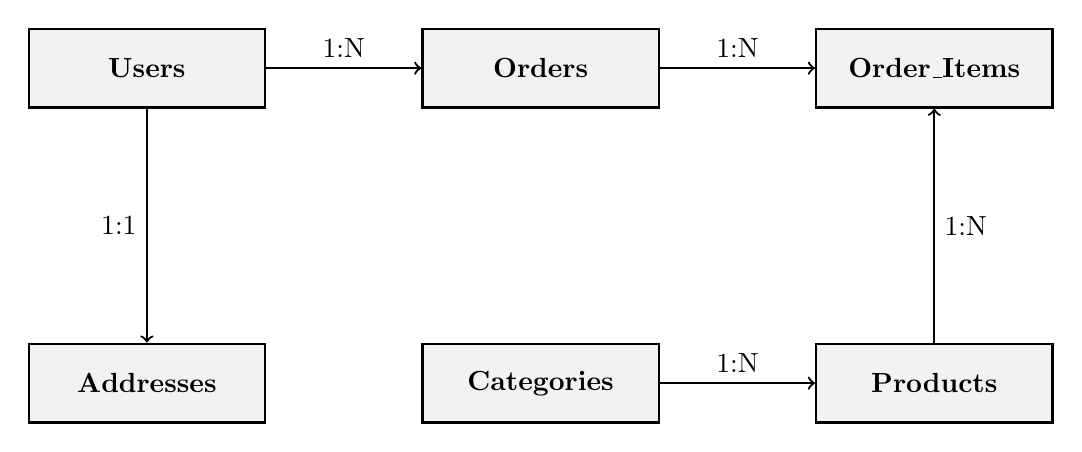
\begin{tikzpicture}[
    entity/.style={rectangle, draw=black, fill=gray!10, thick, minimum width=3cm, minimum height=1cm},
    relationship/.style={diamond, draw=black, fill=gray!20, thick, aspect=2}
]
    % Entities
    \node[entity] (users) at (0,4) {\textbf{Users}};
    \node[entity] (orders) at (5,4) {\textbf{Orders}};
    \node[entity] (orderitems) at (10,4) {\textbf{Order\_Items}};
    \node[entity] (products) at (10,0) {\textbf{Products}};
    \node[entity] (categories) at (5,0) {\textbf{Categories}};
    \node[entity] (addresses) at (0,0) {\textbf{Addresses}};
    
    % Relationships
    \draw[->, thick] (users) -- node[above] {1:N} (orders);
    \draw[->, thick] (orders) -- node[above] {1:N} (orderitems);
    \draw[->, thick] (products) -- node[right] {1:N} (orderitems);
    \draw[->, thick] (categories) -- node[above] {1:N} (products);
    \draw[->, thick] (users) -- node[left] {1:1} (addresses);
\end{tikzpicture}
\caption{Entity Relationship Diagram}
\end{figure}

%=============================================================================
\section{Backend Implementation (PHP)}
%=============================================================================

\subsection{Authentication System}

\subsubsection{Login Process (login.php)}

The login system uses dynamic column detection for database compatibility:

\begin{lstlisting}[language=PHP, caption=Authentication Logic]
<?php
session_start();
require_once '../config/db.php';

if ($_SERVER['REQUEST_METHOD'] === 'POST') {
    $conn = getDBConnection();
    $email = sanitize($_POST['email']);
    $password = $_POST['password'];
    
    // Dynamic column detection for compatibility
    $columnsResult = $conn->query("SHOW COLUMNS FROM users");
    $columns = [];
    while ($col = $columnsResult->fetch_assoc()) {
        $columns[] = $col['Field'];
    }
    
    $hasPasswordHash = in_array('password_hash', $columns);
    $hasIsAdmin = in_array('is_admin', $columns);
    
    // Prepared statement prevents SQL injection
    $stmt = $conn->prepare("SELECT * FROM users WHERE email = ?");
    $stmt->bind_param("s", $email);
    $stmt->execute();
    $result = $stmt->get_result();
    
    if ($result->num_rows === 1) {
        $user = $result->fetch_assoc();
        
        // Secure password verification
        if (password_verify($password, $user['password_hash'])) {
            // Set session variables
            $_SESSION['user_id'] = $user['user_id'];
            $_SESSION['username'] = $user['username'];
            $_SESSION['is_admin'] = $user['is_admin'] ?? 0;
            
            // Role-based redirection
            if ($_SESSION['is_admin'] == 1) {
                header("Location: admin-dashboard.php");
            } else {
                header("Location: index.php");
            }
            exit();
        }
    }
}
?>
\end{lstlisting}

\subsubsection{Session Management}

Sessions are initialized at the top of each protected page:

\begin{lstlisting}[language=PHP, caption=Session Protection Pattern]
<?php
session_start();
require_once '../config/db.php';

// Redirect unauthenticated users
if (!isset($_SESSION['user_id'])) {
    header("Location: login.php?redirect=" . urlencode($_SERVER['REQUEST_URI']));
    exit();
}
?>
\end{lstlisting}

\subsection{CRUD Operations}

\subsubsection{Product Management (manage-products.php)}

Full CRUD implementation with prepared statements:

\begin{lstlisting}[language=PHP, caption=Product CRUD Operations]
<?php
// CREATE - Add new product
case 'add':
    $name = sanitize($_POST['name']);
    $brand = sanitize($_POST['brand']);
    $description = sanitize($_POST['description']);
    $price = floatval($_POST['price']);
    $stock = intval($_POST['stock']);
    $category_id = intval($_POST['category_id']);
    
    $stmt = $conn->prepare(
        "INSERT INTO products (name, brand, description, price, stock, category_id) 
         VALUES (?, ?, ?, ?, ?, ?)"
    );
    $stmt->bind_param("sssdii", $name, $brand, $description, 
                       $price, $stock, $category_id);
    $stmt->execute();
    break;

// READ - Fetch all products with category names
$result = $conn->query(
    "SELECT p.*, 
     (SELECT c.name FROM categories c WHERE c.category_id = p.category_id) 
     as category_name
     FROM products p ORDER BY p.product_id DESC"
);
$products = $result->fetch_all(MYSQLI_ASSOC);

// UPDATE - Edit existing product
case 'edit':
    $product_id = intval($_POST['product_id']);
    $stmt = $conn->prepare(
        "UPDATE products SET name=?, brand=?, description=?, 
         price=?, stock=?, category_id=? WHERE product_id=?"
    );
    $stmt->bind_param("sssdiis", $name, $brand, $description,
                       $price, $stock, $category_id, $product_id);
    $stmt->execute();
    break;

// DELETE - Remove product
case 'delete':
    $product_id = intval($_POST['product_id']);
    $stmt = $conn->prepare("DELETE FROM products WHERE product_id = ?");
    $stmt->bind_param("i", $product_id);
    $stmt->execute();
    break;
?>
\end{lstlisting}

\subsection{Order Processing with Transactions}

The checkout system uses database transactions for data integrity:

\begin{lstlisting}[language=PHP, caption=Transaction-Based Order Processing]
<?php
try {
    // Start transaction - all or nothing
    $conn->begin_transaction();
    
    // Create order record
    $stmt = $conn->prepare(
        "INSERT INTO orders (customer_id, order_date, total_amount, 
         currency, status, shipping_address, notes) 
         VALUES (?, NOW(), ?, 'USD', 'Processing', ?, ?)"
    );
    $stmt->bind_param("idss", $user_id, $total_amount, 
                       $shipping_address, $notes);
    $stmt->execute();
    $order_id = $conn->insert_id;
    
    // Insert order items and reduce stock atomically
    foreach ($cart_items as $item) {
        // Add to order_items
        $stmt_item->bind_param("iiid", $order_id, $product_id, 
                                $quantity, $price);
        $stmt_item->execute();
        
        // Reduce stock with validation
        $stmt_stock = $conn->prepare(
            "UPDATE products SET stock = stock - ? 
             WHERE product_id = ? AND stock >= ?"
        );
        $stmt_stock->bind_param("iii", $quantity, $product_id, $quantity);
        $stmt_stock->execute();
        
        // Rollback if insufficient stock
        if ($stmt_stock->affected_rows === 0) {
            throw new Exception('Insufficient stock');
        }
    }
    
    // Commit only if all operations succeed
    $conn->commit();
    
} catch (Exception $e) {
    // Rollback all changes on error
    $conn->rollback();
    $error_message = $e->getMessage();
}
?>
\end{lstlisting}

%=============================================================================
\section{Frontend Implementation}
%=============================================================================

\subsection{CSS Architecture}

The stylesheet (\texttt{styles.css}, 1400+ lines) uses CSS custom properties (variables) for theming:

\begin{lstlisting}[language=CSS, caption=CSS Variables for Theming]
:root {
    --primary-color: #2563eb;
    --secondary-color: #64748b;
    --accent-color: #f97316;
    --success-color: #10b981;
    --danger-color: #ef4444;
    --dark-color: #1e293b;
    --light-color: #f8fafc;
    --border-color: #e2e8f0;
    --text-primary: #0f172a;
    --text-secondary: #64748b;
    --bg-color: #ffffff;
    --card-bg: #ffffff;
    --shadow-md: 0 4px 6px -1px rgba(0, 0, 0, 0.1);
    --transition: all 0.3s ease;
}

/* Dark Mode Override */
body.dark-mode {
    --primary-color: #3b82f6;
    --text-primary: #f1f5f9;
    --bg-color: #1e293b;
    --card-bg: #334155;
}
\end{lstlisting}

\subsection{Responsive Design}

Five breakpoints ensure optimal display across devices:

\begin{lstlisting}[language=CSS, caption=Responsive Breakpoints]
/* Large Desktop */
@media (max-width: 1200px) {
    .features-grid { grid-template-columns: repeat(2, 1fr); }
}

/* Tablet Landscape */
@media (max-width: 968px) {
    .navbar .container { flex-wrap: wrap; }
    .menu-toggle { display: flex; }
}

/* Tablet Portrait */
@media (max-width: 768px) {
    .nav-links {
        display: none;
        flex-direction: column;
        width: 100%;
    }
    .nav-links.active { display: flex; }
}

/* Mobile */
@media (max-width: 480px) {
    .hero h1 { font-size: 1.75rem; }
    .product-grid { grid-template-columns: 1fr; }
}

/* Small Mobile */
@media (max-width: 360px) {
    .container { padding: 0 10px; }
}
\end{lstlisting}

\subsection{JavaScript Functionality}

\subsubsection{Shopping Cart Implementation}

The cart uses localStorage for persistence across sessions:

\begin{lstlisting}[language=JavaScript, caption=Shopping Cart Logic]
// Initialize cart from localStorage
let cart = JSON.parse(localStorage.getItem("cart")) || [];

// Add to cart with notification
document.querySelectorAll(".add-to-cart-btn").forEach((button) => {
    button.addEventListener("click", function (e) {
        e.preventDefault();
        
        const item = {
            id: this.dataset.id,
            name: this.dataset.name,
            price: this.dataset.price,
            quantity: 1,
            icon: this.dataset.icon
        };
        
        // Add to cart array
        cart.push(item);
        
        // Persist to localStorage
        localStorage.setItem("cart", JSON.stringify(cart));
        
        // Update UI
        updateCart();
        showNotification("Product added to cart!", "#10b981");
    });
});

// Calculate and display cart total
function updateCart() {
    cartCount.textContent = cart.length;
    
    let total = cart.reduce((sum, item) => 
        sum + (parseFloat(item.price) * item.quantity), 0);
    
    cartTotal.textContent = `$${total.toLocaleString()}`;
}
\end{lstlisting}

\subsubsection{Dark Mode Toggle}

\begin{lstlisting}[language=JavaScript, caption=Dark Mode Implementation]
const darkModeToggle = document.getElementById("darkModeToggle");
const body = document.body;

// Check saved preference
if (localStorage.getItem("darkMode") === "enabled") {
    body.classList.add("dark-mode");
}

darkModeToggle.addEventListener("click", function () {
    body.classList.toggle("dark-mode");
    
    const isDark = body.classList.contains("dark-mode");
    localStorage.setItem("darkMode", isDark ? "enabled" : "disabled");
    
    // Update icon
    this.querySelector(".icon").textContent = isDark ? "sun" : "moon";
});
\end{lstlisting}

\subsubsection{Dynamic Navigation}

Navigation adapts based on authentication status:

\begin{lstlisting}[language=PHP, caption=Dynamic Navigation (PHP)]
<ul class="nav-links" id="navLinks">
    <li><a href="index.php">Home</a></li>
    <li><a href="products.php">Products</a></li>
    
    <?php if (isset($_SESSION['user_id'])): ?>
        <!-- Authenticated users see Profile/Logout -->
        <li><a href="profile.php">Profile</a></li>
        <li><a href="logout.php">Logout</a></li>
    <?php else: ?>
        <!-- Guests see Login -->
        <li><a href="login.php">Login</a></li>
    <?php endif; ?>
    
    <li><a href="checkout.php">Checkout</a></li>
</ul>
\end{lstlisting}

%=============================================================================
\section{Security Measures}
%=============================================================================

\subsection{SQL Injection Prevention}

All database queries use prepared statements with parameterized queries:

\begin{lstlisting}[language=PHP, caption=Prepared Statement Example]
// UNSAFE (vulnerable to SQL injection)
// $query = "SELECT * FROM users WHERE email = '$email'";

// SAFE (parameterized query)
$stmt = $conn->prepare("SELECT * FROM users WHERE email = ?");
$stmt->bind_param("s", $email);  // "s" = string type
$stmt->execute();
\end{lstlisting}

\subsection{XSS Prevention}

User input is sanitized before display:

\begin{lstlisting}[language=PHP, caption=Input Sanitization]
function sanitize($data) {
    // Remove whitespace
    $data = trim($data);
    // Remove HTML tags
    $data = strip_tags($data);
    // Convert special characters to HTML entities
    $data = htmlspecialchars($data, ENT_QUOTES, 'UTF-8');
    return $data;
}

// Usage in output
echo htmlspecialchars($user['username']);
\end{lstlisting}

\subsection{Password Security}

Passwords are hashed using PHP's built-in bcrypt:

\begin{lstlisting}[language=PHP, caption=Password Hashing]
// During registration
$password_hash = password_hash($password, PASSWORD_DEFAULT);

// During login
if (password_verify($input_password, $stored_hash)) {
    // Password matches
}
\end{lstlisting}

\subsection{Session Security}

\begin{itemize}
    \item Sessions are started with \texttt{session\_start()} on each page
    \item Session variables store user ID, not sensitive data
    \item Logout properly destroys the session:
\end{itemize}

\begin{lstlisting}[language=PHP, caption=Secure Logout]
<?php
session_start();
session_unset();      // Clear all session variables
session_destroy();    // Destroy the session
header("Location: index.php");
exit();
?>
\end{lstlisting}

%=============================================================================
\section{Admin Panel Features}
%=============================================================================

\subsection{Dashboard Statistics}

The admin dashboard displays real-time statistics:

\begin{lstlisting}[language=PHP, caption=Dashboard Statistics Queries]
// Total Products
$result = $conn->query("SELECT COUNT(*) as total FROM products");
$totalProducts = $result->fetch_assoc()['total'];

// Total Orders
$result = $conn->query("SELECT COUNT(*) as total FROM orders");
$totalOrders = $result->fetch_assoc()['total'];

// Total Revenue
$result = $conn->query(
    "SELECT COALESCE(SUM(total_amount), 0) as revenue FROM orders"
);
$revenue = $result->fetch_assoc()['revenue'];

// Total Users
$result = $conn->query("SELECT COUNT(*) as total FROM users");
$totalUsers = $result->fetch_assoc()['total'];

// Total Categories
$result = $conn->query("SELECT COUNT(*) as total FROM categories");
$totalCategories = $result->fetch_assoc()['total'];
\end{lstlisting}

\subsection{Order Management}

Admins can update order statuses through a modal interface:

\begin{lstlisting}[language=PHP, caption=Order Status Update]
if ($_POST['action'] === 'update_status') {
    $order_id = intval($_POST['order_id']);
    $status = sanitize($_POST['status']);
    
    $stmt = $conn->prepare(
        "UPDATE orders SET status = ? WHERE order_id = ?"
    );
    $stmt->bind_param("si", $status, $order_id);
    $stmt->execute();
}
\end{lstlisting}

Available status options:
\begin{itemize}
    \item Pending
    \item Processing
    \item Shipped
    \item Completed
    \item Cancelled
\end{itemize}

%=============================================================================
\section{User Features}
%=============================================================================

\subsection{Profile Management}

Users can view and update their address information:

\begin{lstlisting}[language=PHP, caption=Profile Update Logic]
// Fetch user with address (LEFT JOIN handles missing addresses)
$stmt = $conn->prepare(
    "SELECT u.username, u.email, a.street, a.city, a.country, a.postal_code 
     FROM users u 
     LEFT JOIN addresses a ON u.user_id = a.user_id 
     WHERE u.user_id = ?"
);

// Handle profile update (INSERT or UPDATE)
if ($result->num_rows > 0) {
    // Update existing address
    $stmt = $conn->prepare(
        "UPDATE addresses SET street=?, city=?, country=?, postal_code=? 
         WHERE user_id=?"
    );
} else {
    // Create new address
    $stmt = $conn->prepare(
        "INSERT INTO addresses (user_id, street, city, country, postal_code) 
         VALUES (?, ?, ?, ?, ?)"
    );
}
\end{lstlisting}

\subsection{Order History}

Users can view their order history with order items:

\begin{lstlisting}[language=PHP, caption=Order History Query]
// Fetch user's orders only
$result = $conn->query(
    "SELECT o.order_id, o.order_date, o.total_amount, o.status, 
            o.shipping_address 
     FROM orders o 
     WHERE o.customer_id = $user_id 
     ORDER BY o.order_date DESC"
);

// Fetch items for each order
$items_result = $conn->query(
    "SELECT oi.quantity, oi.price, p.name 
     FROM order_items oi 
     LEFT JOIN products p ON oi.product_id = p.product_id 
     WHERE oi.order_id = " . $order['order_id']
);
\end{lstlisting}

%=============================================================================
\section{Installation Guide}
%=============================================================================

\subsection{Prerequisites}

\begin{itemize}
    \item \textbf{Web Server:} Apache 2.4+ (via XAMPP, WAMP, or standalone)
    \item \textbf{PHP:} Version 7.4 or higher with MySQLi extension
    \item \textbf{Database:} MySQL 5.7+ or MariaDB 10.4+
    \item \textbf{Browser:} Modern browser (Chrome, Firefox, Edge, Safari)
\end{itemize}

\subsection{Installation Steps}

\begin{enumerate}
    \item \textbf{Clone the Repository:}
    \begin{lstlisting}[language=bash]
git clone https://github.com/Magdy-00/Web-Technology-Project.git
cd Web-Technology-Project
git checkout Mego
    \end{lstlisting}
    
    \item \textbf{Configure Database:}
    \begin{itemize}
        \item Open phpMyAdmin (\texttt{http://localhost/phpmyadmin})
        \item Create database: \texttt{computer\_clowns}
        \item Import: \texttt{assets/sql/computer\_clowns.sql}
    \end{itemize}
    
    \item \textbf{Update Configuration:}
    Edit \texttt{config/db.php} if needed:
    \begin{lstlisting}[language=PHP]
define('DB_HOST', 'localhost');
define('DB_USER', 'root');
define('DB_PASS', '');  // Add password if set
define('DB_NAME', 'computer_clowns');
    \end{lstlisting}
    
    \item \textbf{Deploy to Web Server:}
    \begin{itemize}
        \item Copy project to \texttt{htdocs/project/} (XAMPP) or \texttt{www/project/} (WAMP)
    \end{itemize}
    
    \item \textbf{Access Application:}
    \begin{itemize}
        \item Home: \texttt{http://localhost/project/html/index.php}
        \item Admin: Login with admin credentials
    \end{itemize}
\end{enumerate}

\subsection{Default Credentials}

\begin{table}[H]
\centering
\begin{tabular}{@{}lll@{}}
\toprule
\textbf{Role} & \textbf{Email} & \textbf{Password} \\
\midrule
Admin & admin@techmart.com & admin123 \\
\bottomrule
\end{tabular}
\caption{Default Login Credentials}
\end{table}

%=============================================================================
\section{File Reference}
%=============================================================================

\begin{longtable}{@{}p{4cm}p{10cm}@{}}
\toprule
\textbf{File} & \textbf{Description} \\
\midrule
\endhead

\multicolumn{2}{l}{\textbf{Configuration}} \\
\midrule
config/db.php & Database connection, sanitization functions \\
\midrule

\multicolumn{2}{l}{\textbf{Public Pages}} \\
\midrule
html/index.php & Home page with hero, features, categories \\
html/products.php & Product catalog with filtering \\
html/login.php & User authentication form \\
html/signup.php & User registration form \\
html/logout.php & Session termination \\
html/checkout.php & Order placement (requires login) \\
html/order-history.php & User's orders (requires login) \\
html/profile.php & User profile/address management \\
html/wishlist.php & Product wishlist \\
\midrule

\multicolumn{2}{l}{\textbf{Admin Pages}} \\
\midrule
html/admin-dashboard.php & Statistics overview \\
html/manage-products.php & Product CRUD interface \\
html/manage-orders.php & Order status management \\
\midrule

\multicolumn{2}{l}{\textbf{Assets}} \\
\midrule
assets/css/styles.css & Main stylesheet (1400+ lines) \\
assets/js/script.js & Client-side JavaScript (400+ lines) \\
assets/sql/computer\_clowns.sql & Database schema and sample data \\
\bottomrule

\caption{Complete File Reference}
\end{longtable}

%=============================================================================
\section{API Endpoints (Form Actions)}
%=============================================================================

The application uses traditional form submissions rather than REST APIs:

\begin{table}[H]
\centering
\begin{tabular}{@{}llll@{}}
\toprule
\textbf{Page} & \textbf{Method} & \textbf{Action} & \textbf{Parameters} \\
\midrule
login.php & POST & Authenticate & email, password \\
signup.php & POST & Register & username, email, password \\
checkout.php & POST & Place Order & fullname, address, cart\_items \\
profile.php & POST & Update Profile & street, city, country, postal\_code \\
manage-products.php & POST & Add Product & name, brand, price, stock, etc. \\
manage-products.php & POST & Edit Product & product\_id, name, price, etc. \\
manage-products.php & POST & Delete Product & product\_id \\
manage-orders.php & POST & Update Status & order\_id, status \\
\bottomrule
\end{tabular}
\caption{Form Action Reference}
\end{table}

%=============================================================================
\section{Conclusion}
%=============================================================================

TechMart represents a complete, production-ready e-commerce solution built with fundamental web technologies. The application demonstrates:

\begin{itemize}
    \item \textbf{Clean Architecture:} Organized file structure with separation of concerns
    \item \textbf{Security Best Practices:} Prepared statements, input sanitization, password hashing
    \item \textbf{Responsive Design:} Mobile-first CSS with 5 breakpoints
    \item \textbf{Modern UX:} Dark mode, persistent cart, smooth animations
    \item \textbf{Complete CRUD:} Full product and order management
    \item \textbf{Transaction Safety:} Atomic order processing with rollback support
\end{itemize}

The codebase is well-suited for educational purposes, demonstrating core web development concepts, and can serve as a foundation for more complex e-commerce applications.

\end{document}
